\begin{frame}
  \frametitle{2-D Neutronics Quarter-Core \& Full-Core MSRE Models}
  \begin{columns}
    \column{5.5cm}
  \begin{figure}[htb!]
    \centering
    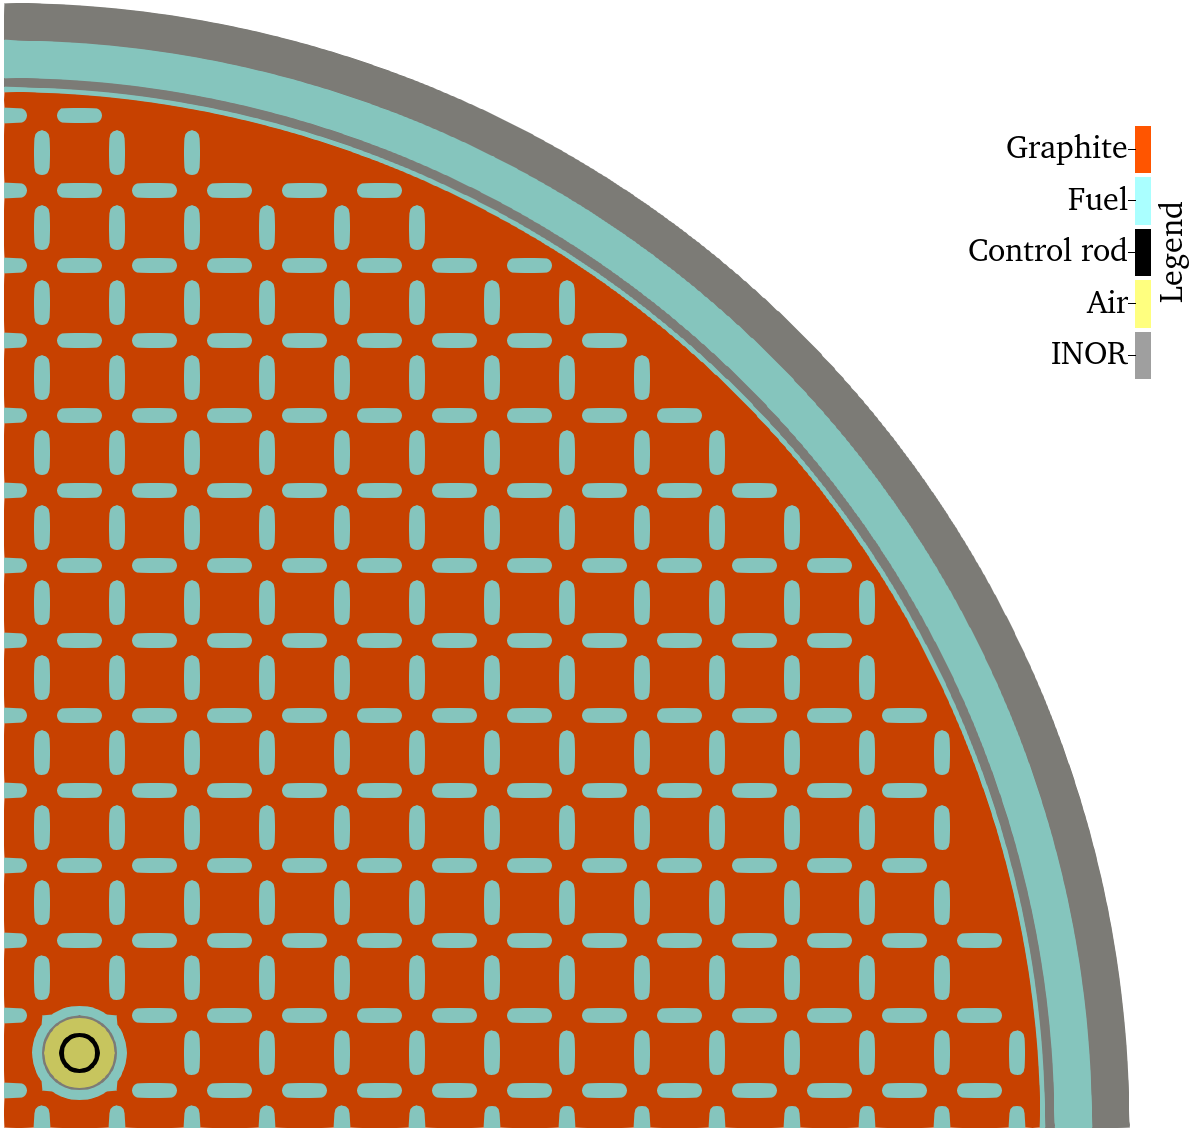
\includegraphics[width=\columnwidth]{quarter-core-geom}
    \caption{2-D \gls{MSRE} quarter-core model based on the horizontal cross section of the actual
    \gls{MSRE} geometry.}
    \label{fig:1/4-geom}
  \end{figure}
  \column{5.5cm}
  \begin{figure}[htb!]
    \centering
    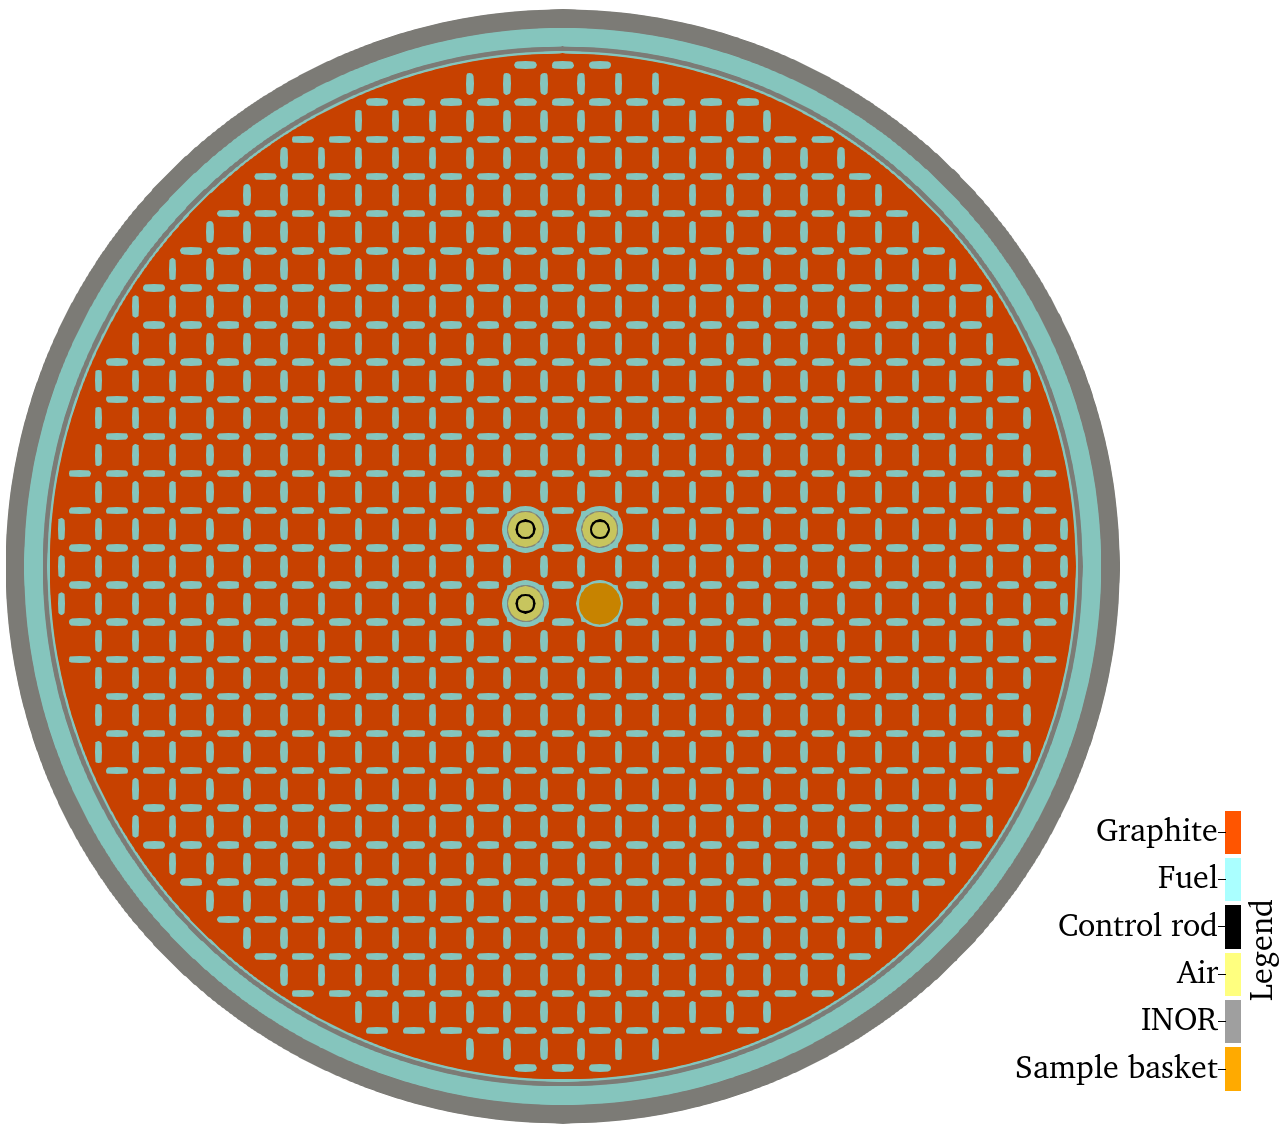
\includegraphics[width=\columnwidth]{full-core-geom}
    \caption{2-D \gls{MSRE} full-core model based on the horizontal cross section of the actual
    \gls{MSRE} geometry.}
    \label{fig:full-geom}
  \end{figure}
\end{columns}
\end{frame}

\begin{frame}
  \frametitle{2-D MSRE Neutronics Modeling Approach}
  \begin{columns}
    \column{6.5cm}
    \textbf{2-D Neutronics MSRE Model Setup}
    \vspace{.2cm}

    Geometry approximations:
    \begin{itemize}
      \item Modeled the control rods as perfectly annular cylinders
      \item Homogenized the nickel alloy, graphite, and molten salt regions in the sample basket
      \item Neglected the thermal insulation and shield structures outside the core
      \item Replaced partial fuel channels and jagged graphite edges on the core periphery
    \end{itemize}
    All material compositions correspond to the original MSRE specifications at initial criticality.
    \column{4.5cm}
    \begin{figure}[htb!]
      \centering
      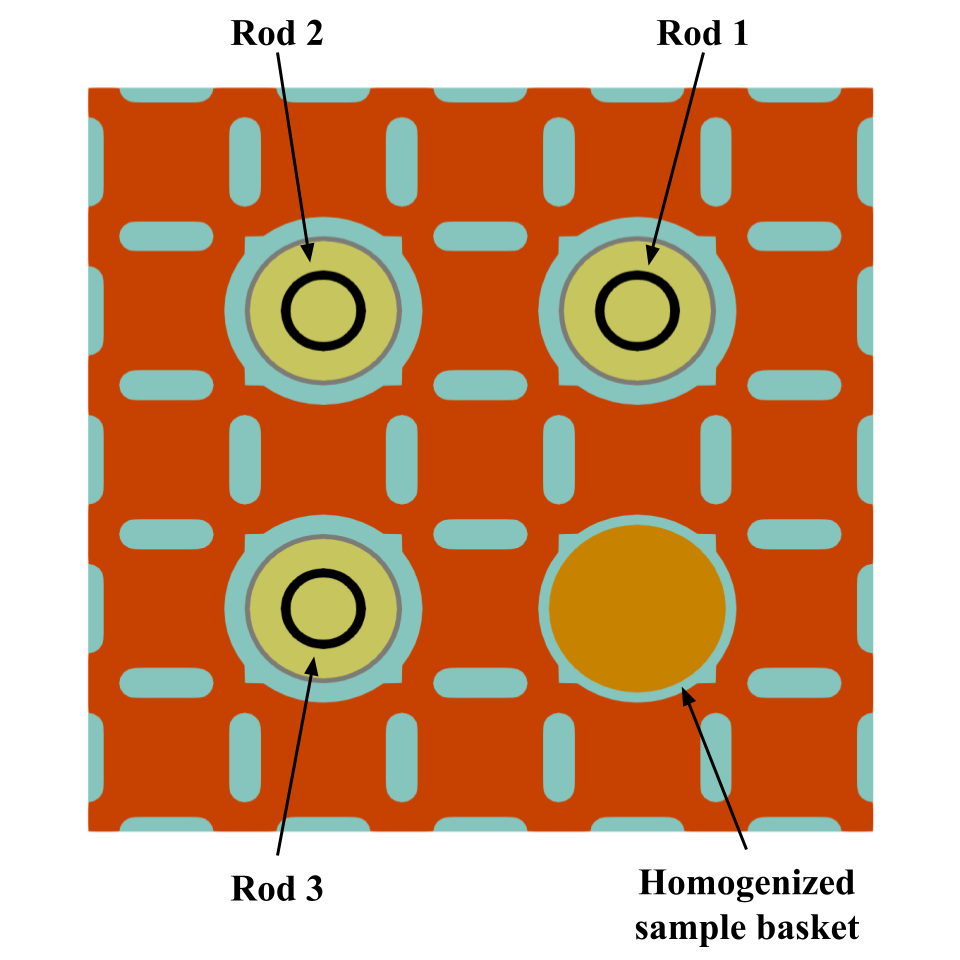
\includegraphics[width=\columnwidth]{full-core-closeup}
      \caption{Detailed view of the control rod thimbles and sample basket in 2-D \gls{MSRE} full-core
        model.}
      \label{fig:full-geom-closeup}
    \end{figure}
  \end{columns}
\end{frame}

\begin{frame}
  \frametitle{2-D MSRE Neutronics Simulation Results}
  \textbf{2-D Quarter-Core $\bm{k}$ \& Rod Worth Results}
  \begin{table}[htb]
    \small
    \centering
    \caption{$k_\text{eff}$ and control rod worth estimates for the 2-D quarter-core \gls{MSRE}
      model. Error values are relative to OpenMC-CE.}
    \setlength\tabcolsep{2pt}
    \begin{tabular}{l S[table-format=1.5(2)] S S[table-format=1.5(2)] S S[table-format=4(2)] S}
      \toprule
      \multirow{2}{*}{Method} & \multicolumn{2}{c}{No Rod} & \multicolumn{2}{c}{Rod} & \multicolumn{2}{c}{Rod worth} \\
                              & {$k_\text{eff}$} & {Error [pcm]} & {$k_\text{eff}$} & {Error [pcm]} & {$\Delta\rho_\text{worth}$ [pcm]} & {Error [pcm]} \\
                              \cmidrule(r){1-1} \cmidrule(rl){2-3} \cmidrule(rl){4-5} \cmidrule(l){6-7}
  	  OpenMC-CE & 1.11209(43) & {-} & 1.01740(42) & {-} & 8370(53) & {-} \\
  	  OpenMC-MG & 1.11979(42) & 618 & 1.02204(41) & 446 & 8541(51) & 172 \\
        Diffusion & 1.12059 & 682 & 1.00903 & -816 & 9867 & 1484 \\
        Hybrid & 1.12174 & 773 & 1.02532 & 760 & 8383 & 13 \\
      \bottomrule
    \end{tabular}
    \label{table:quarter-core}
  \end{table}
  \vspace{.2cm}

  $\Rightarrow$ The hybrid method produces accurate rod worth estimates while the neutron diffusion method
      significantly overestimates rod worth.
\end{frame}

\begin{frame}
%  \frametitle{Hybrid $S_N$-Diffusion Method: 2-D Neutronics Eigenvalue Simulations}
%  \textbf{Normalized Fuel Channel Power Distribution}
  \begin{columns}
    \column{6cm}
    \centerline{\large \textbf{Control Rod Withdrawn}}
  \begin{figure}[p]
    \centering
    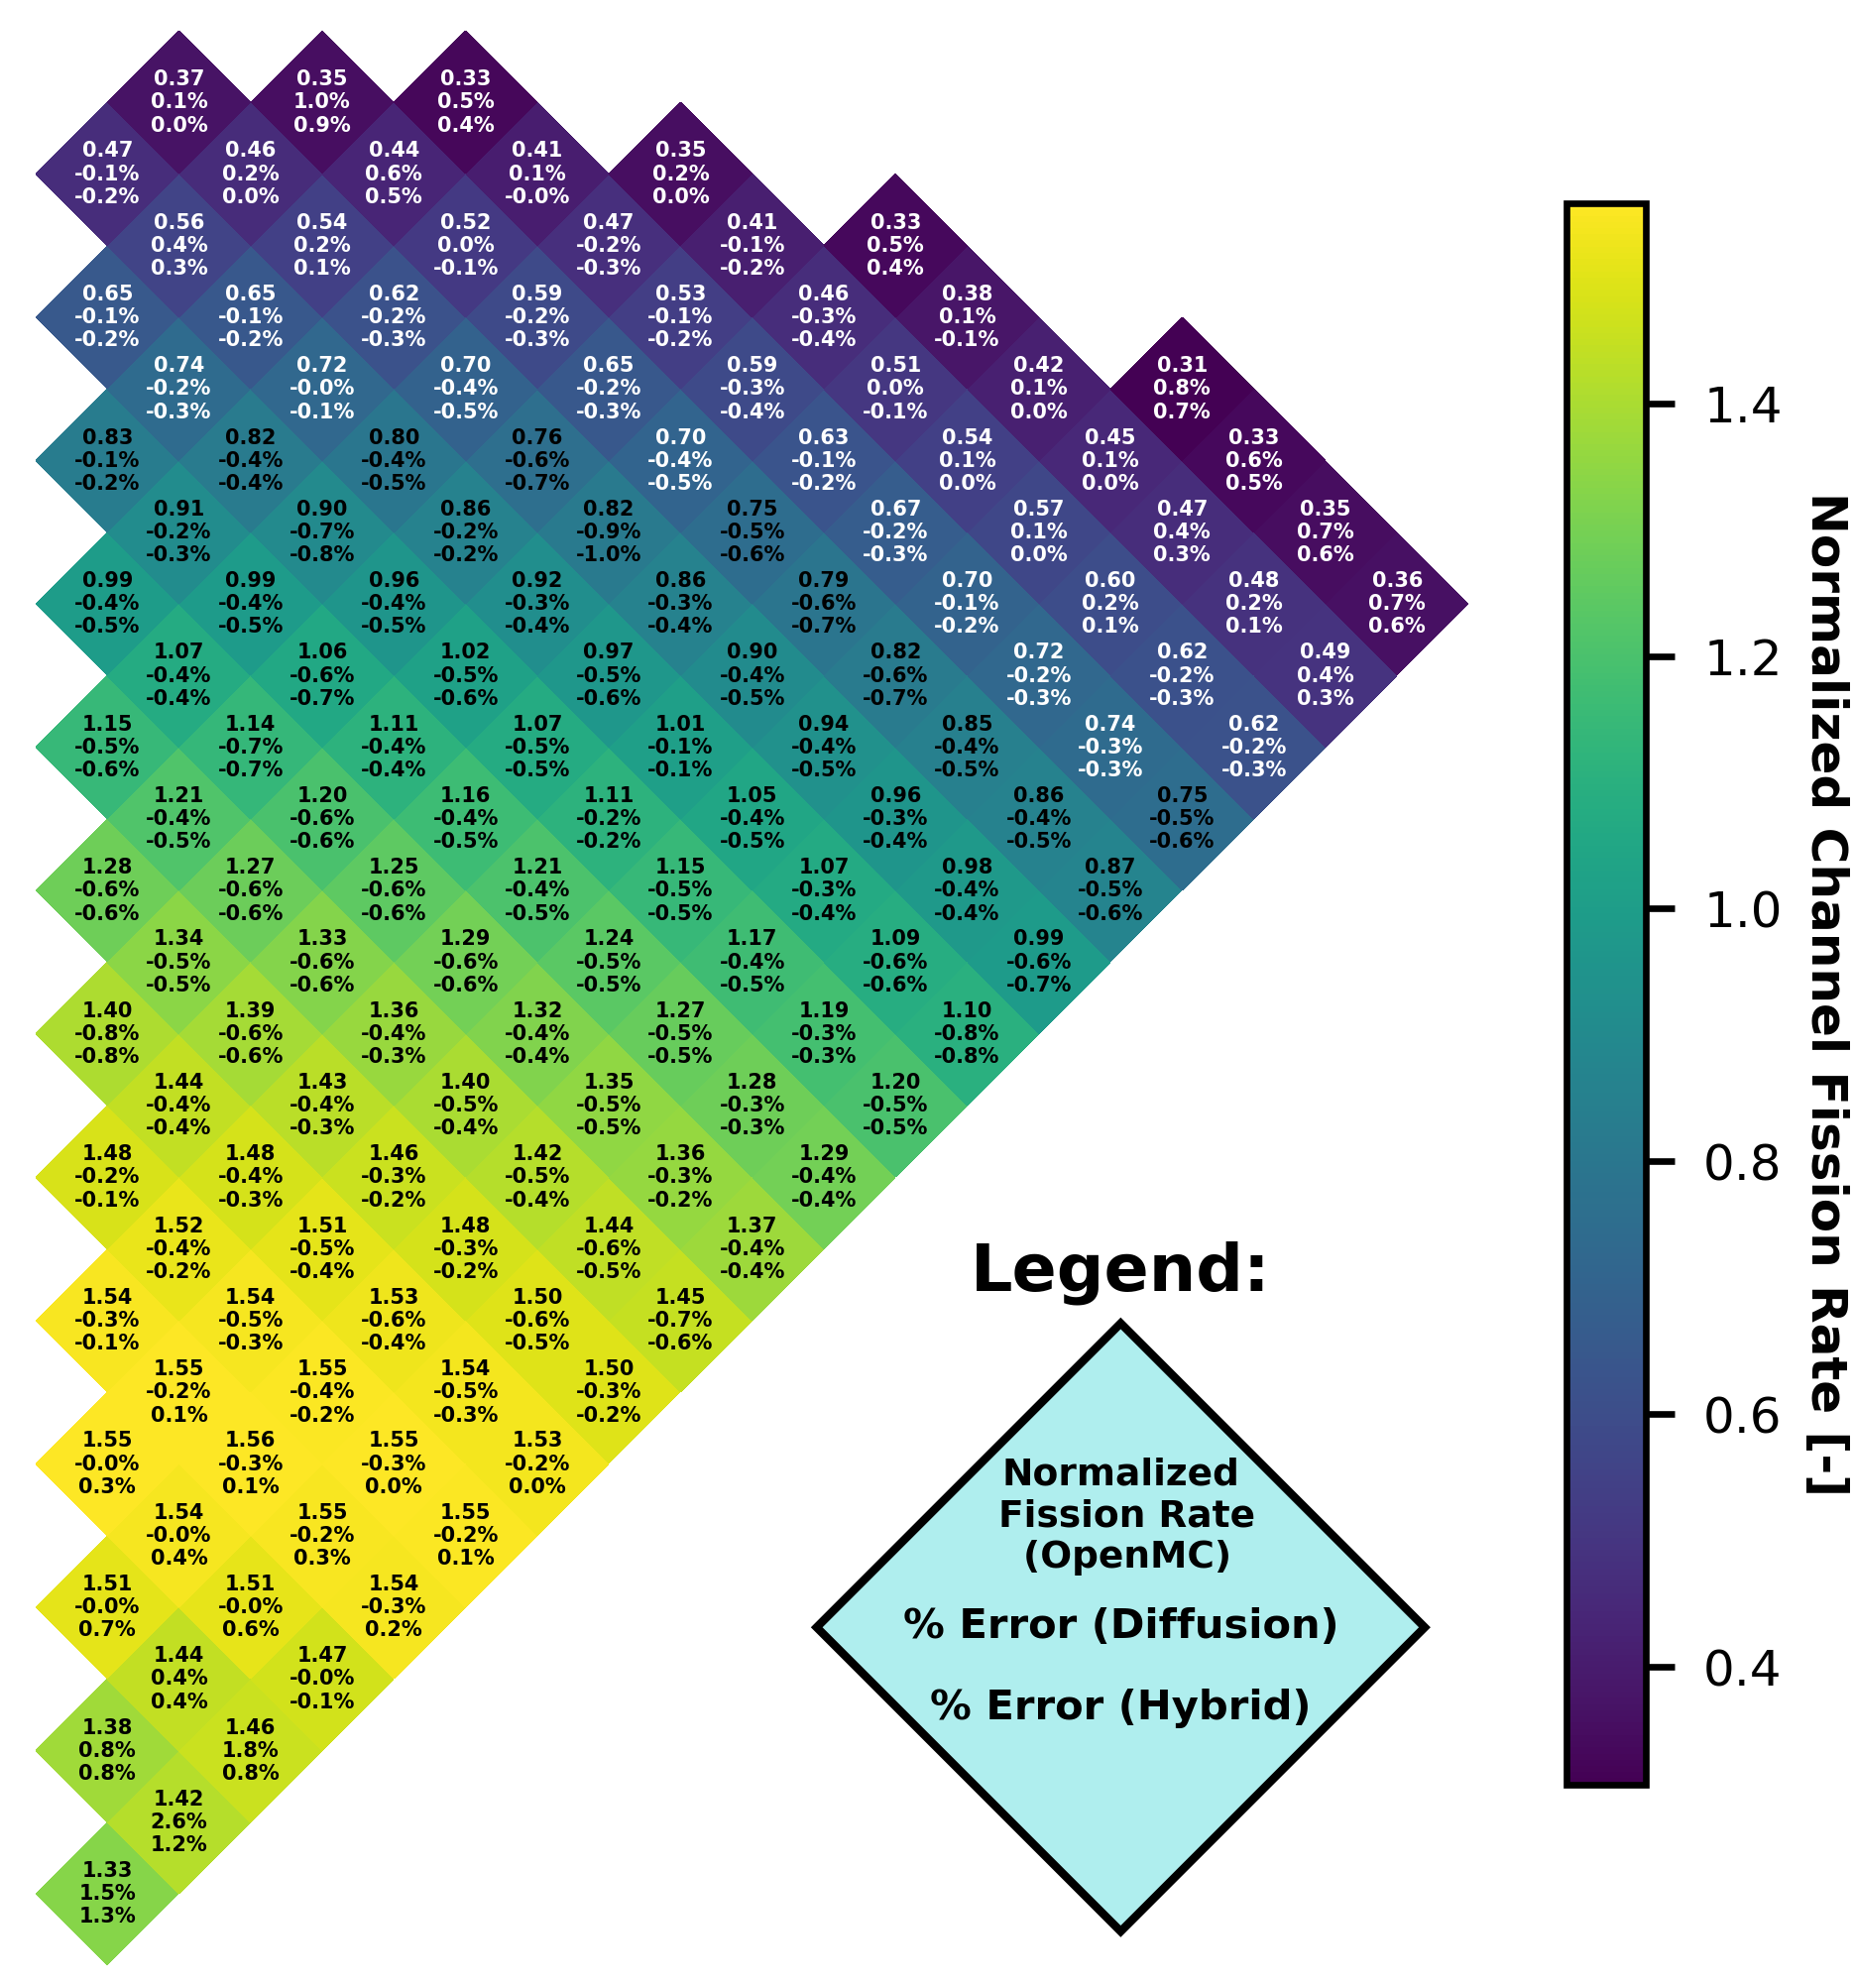
\includegraphics[width=\columnwidth]{msre-quarter-no-rod-power}
    \caption{Normalized channel fission rate distribution of the 2-D \gls{MSRE} quarter-core model
    with the rod withdrawn.}
    \label{fig:1/4-no-rod}
  \end{figure}
    \column{6cm}
    \centerline{\large \textbf{Control Rod Inserted}}
  \begin{figure}[p]
    \centering
    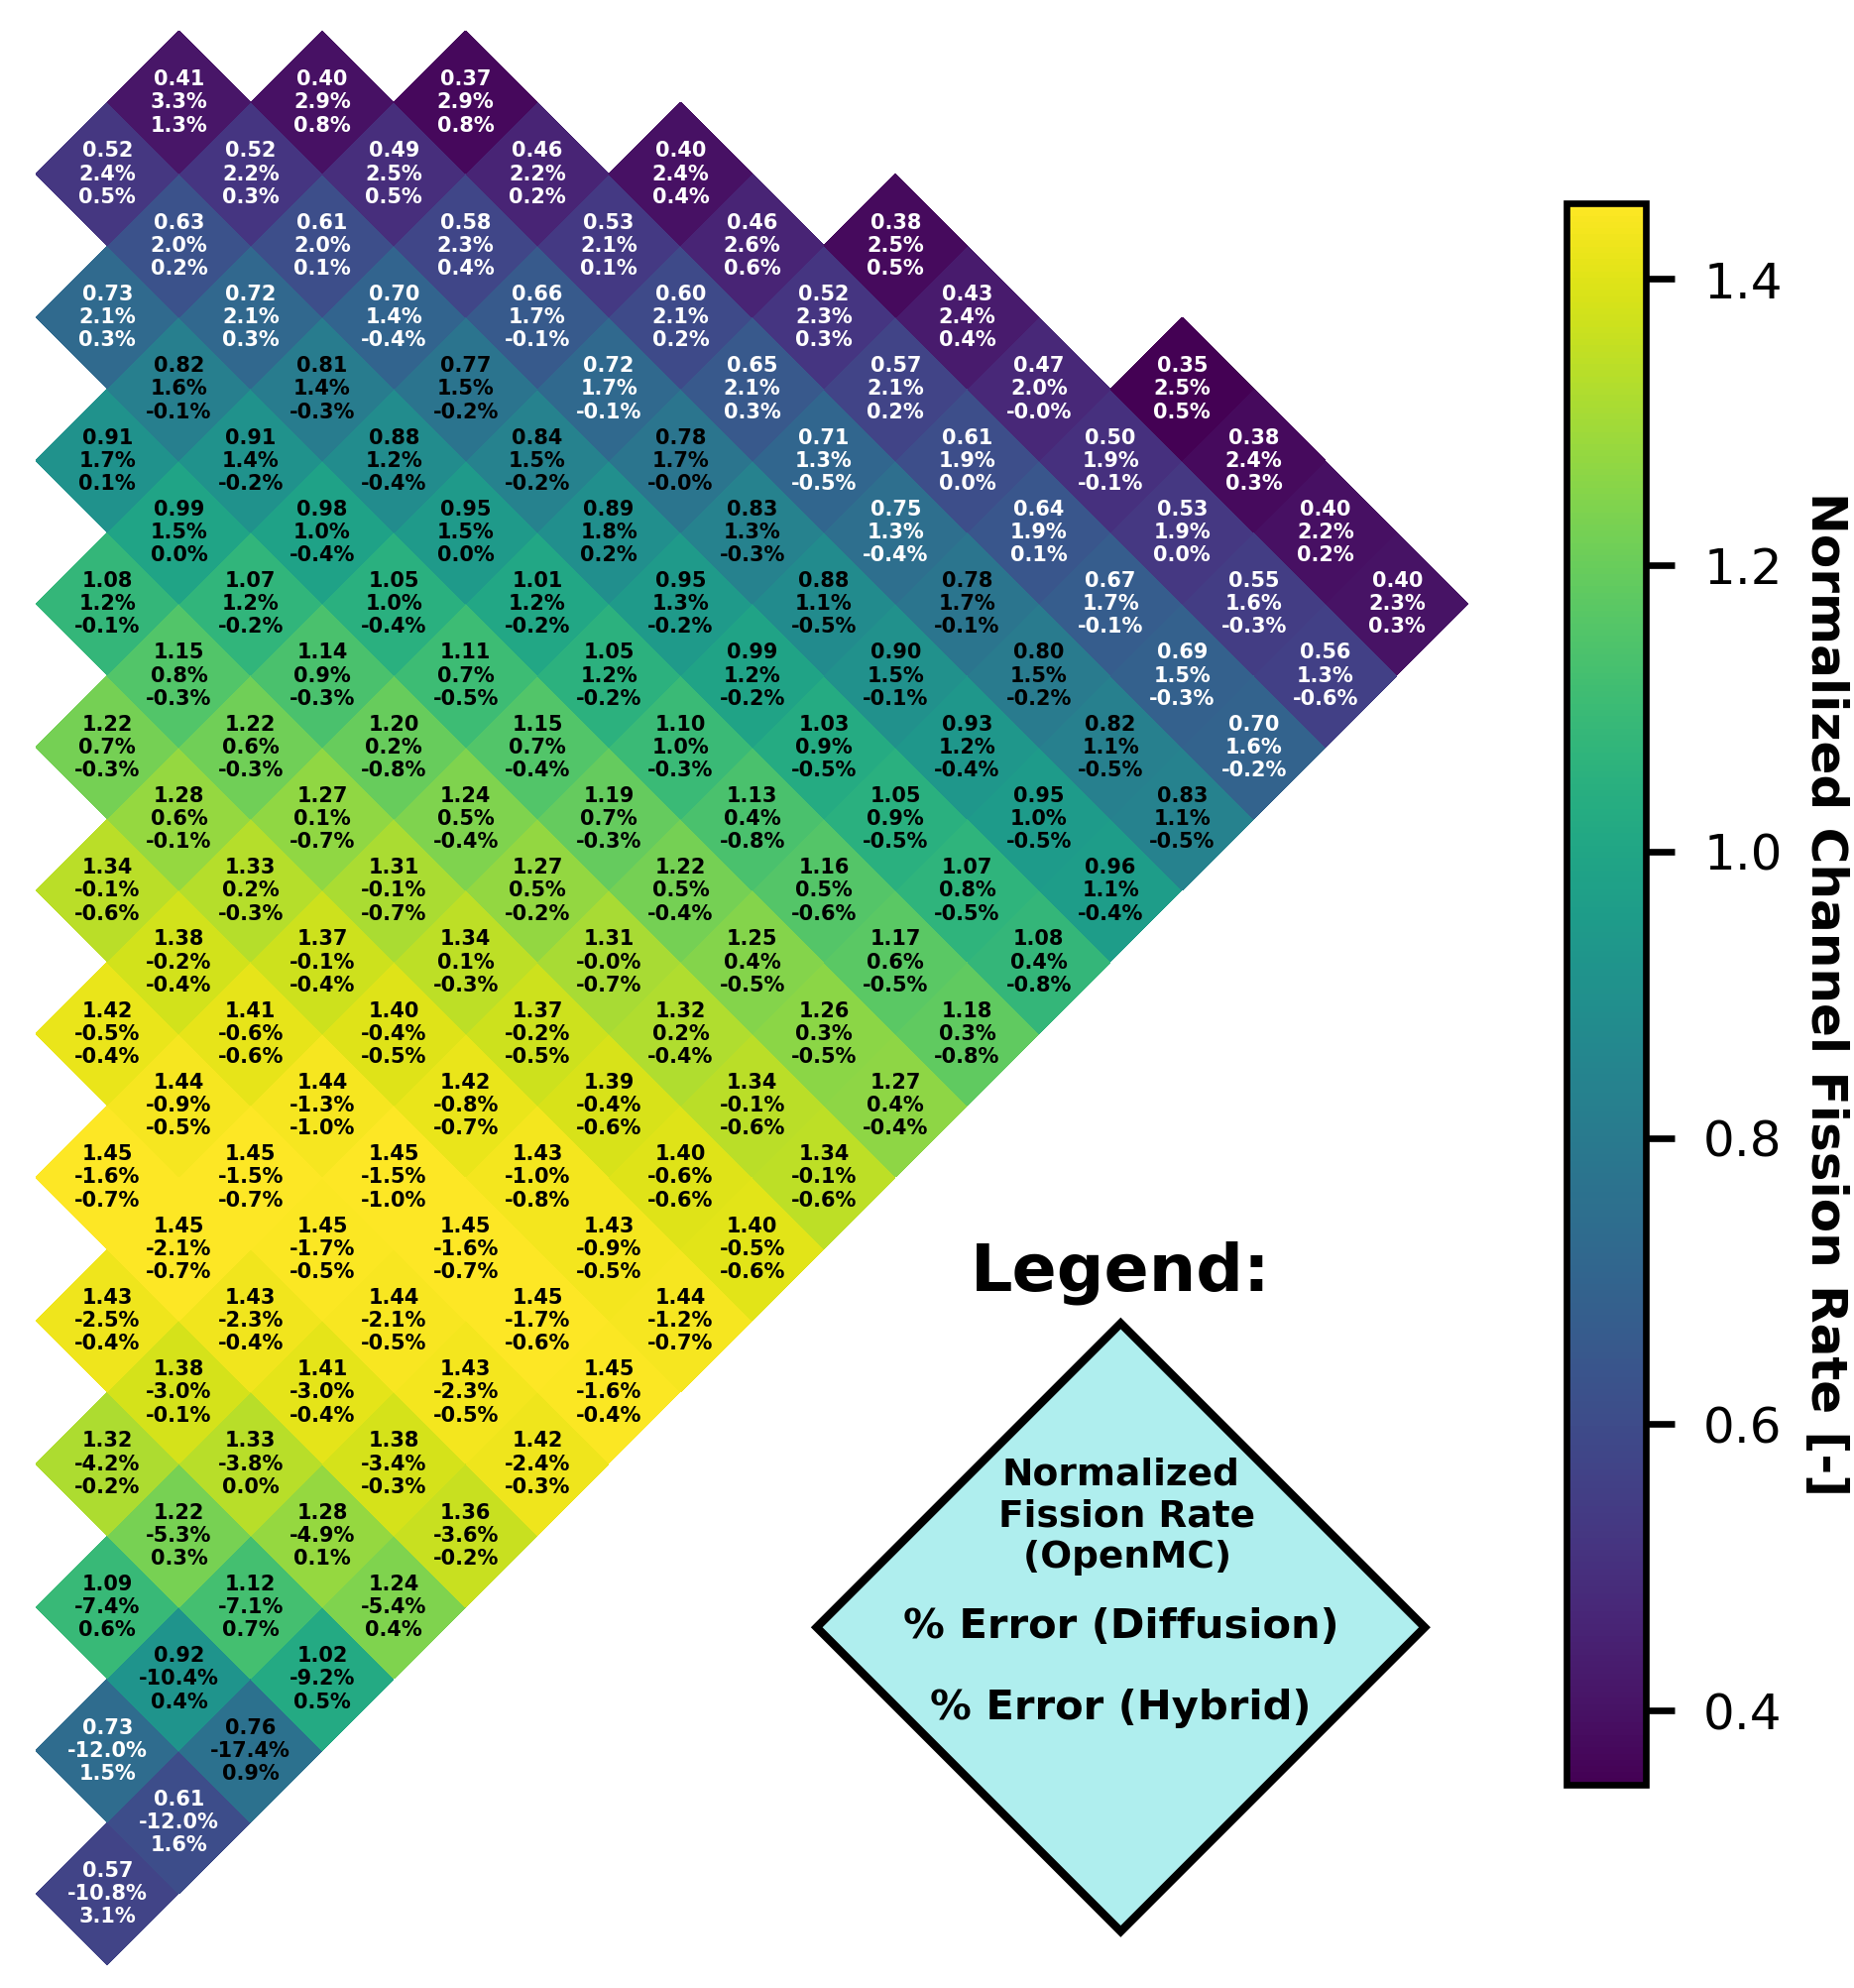
\includegraphics[width=\columnwidth]{msre-quarter-rod-power}
    \caption{Normalized channel fission rate distribution of the 2-D \gls{MSRE} quarter-core model
    with the rod inserted.}
    \label{fig:1/4-rod}
  \end{figure}
\end{columns}
\end{frame}

\begin{frame}
  \frametitle{2-D MSRE Neutronics Simulation Results}
  \textbf{2-D Quarter-Core Normalized Channel Fission Rate Distribution}
  \begin{table}[htb]
    \small
    \centering
    \caption{Absolute mean and maximum percentage errors in the normalized channel fission rates of
    the 2-D \gls{MSRE} quarter-core models relative to OpenMC. The mean relative standard deviation of
    OpenMC normalized channel fission rates is 0.20\%.}
    \begin{tabular}{l S S S S}
      \toprule
      \multirow{2}{*}{Method} & \multicolumn{2}{c}{No Rod} & \multicolumn{2}{c}{Rod} \\
                              & {Mean [\%]} & {Maximum [\%]} & {Mean [\%]} & {Maximum [\%]} \\
                              \cmidrule(r){1-1} \cmidrule(rl){2-3} \cmidrule(l){4-5}
      Diffusion & 0.40 & 2.63 & 2.01 & 17.44 \\
      Hybrid & 0.40 & 1.32 & 0.43 & 3.08 \\
      \bottomrule
    \end{tabular}
    \label{table:quarter-core-power}
  \end{table}
  \vspace{.2cm}

  \begin{itemize}
    \item The hybrid method improves channel fission rate estimates, especially for the rodded case.
    \item Significant improvement in maximum percentage error of the channel fission rate.
  \end{itemize}
\end{frame}

\begin{frame}
  \frametitle{2-D MSRE Neutronics Simulation Results}
  \textbf{2-D Full-Core Rod Worth Results}
  \begin{table}[htb]
    \small
    \centering
    \caption{Control rod worth estimates for the 2-D full-core \gls{MSRE} with the
    indicated rods inserted. Error values are relative to OpenMC-CE.}
    \setlength\tabcolsep{2pt}
    \begin{tabular}{l S[table-format=4(2)] S S[table-format=4(2)] S S[table-format=4(2)] S}
      \toprule
      \multirow{2}{*}{Method} & \multicolumn{2}{c}{Rod 1} & \multicolumn{2}{c}{Rod 1 \& 2} & \multicolumn{2}{c}{Rod 1, 2 \& 3} \\
                              & {$\Delta\rho_\text{worth}$ [pcm]} & {Error [pcm]} & {$\Delta\rho_\text{worth}$ [pcm]} & {Error [pcm]} & {$\Delta\rho_\text{worth}$ [pcm]} & {Error [pcm]} \\
                              \cmidrule(r){1-1} \cmidrule(rl){2-3} \cmidrule(rl){4-5} \cmidrule(l){6-7}
      OpenMC-CE & 2450(25) & {-} & 4494(23) & {-} & 6357(24) & {-} \\
      OpenMC-MG & 2523(23) & 73 & 4640(24) & 146 & 6455(22) & 98 \\
      Diffusion & 3019 & 569 & 5439 & 945 & 7519 & 1162 \\
      Hybrid & 2455 & 5 & 4521 & 27 & 6323 & -34 \\
      \bottomrule
    \end{tabular}
    \label{table:full-core-worth}
  \end{table}
  \vspace{.2cm}

  $\Rightarrow$ The hybrid method remains effective at improving control rod worth estimates in the full-core
  model.
\end{frame}

\begin{frame}
  \frametitle{2-D MSRE Neutronics Simulation Results}
  \textbf{2-D Full-Core Normalized Channel Fission Rate Distribution}
  \begin{table}[htb]
    \footnotesize
    \centering
    \caption{Absolute mean and maximum percentage errors in the normalized channel fission rates of
    the 2-D \gls{MSRE} full-core models relative to OpenMC. The mean relative standard deviation of
    OpenMC normalized channel fission rates is 0.27\%.}
    \setlength\tabcolsep{1pt}
    \begin{tabular}{l S S S S S S S S}
      \toprule
      \multirow{2}{*}{Method} & \multicolumn{2}{c}{No Rod} & \multicolumn{2}{c}{Rod 1} & \multicolumn{2}{c}{Rod 1 \& 2} & \multicolumn{2}{c}{Rod 1, 2 \& 3} \\
                              & {Mean [\%]} & {Maximum [\%]} & {Mean [\%]} & {Maximum [\%]} & {Mean [\%]} & {Maximum [\%]} & {Mean [\%]} & {Maximum [\%]} \\
                              \cmidrule(r){1-1} \cmidrule(rl){2-3} \cmidrule(rl){4-5} \cmidrule(rl){6-7} \cmidrule(l){8-9}
      Diffusion & 0.45 & 2.95 & 0.94 & 12.61 & 1.35 & 15.34 & 1.67 & 17.09 \\
      Hybrid & 0.43 & 1.45 & 0.43 & 1.82 & 0.43 & 2.26 & 0.43 & 2.52 \\
      \bottomrule
    \end{tabular}
    \label{table:full-core-power}
  \end{table}
  \vspace{.2cm}

  \begin{itemize}
    \item Mean percentage error for the hybrid method remains consistent at 0.43\%.
    \item Significant improvement in maximum percentage error of the channel fission rate.
  \end{itemize}
\end{frame}
